\section{Evaluation} \label{evaluation}

We evaluated Neptune against Julia on a computer with 16 GB RAM and an Intel Core i7-4790 CPU with 8 cores reported to the OS, a frequency of up to $3.60$~GHz, and 32KB, 256KB, 8MB L1, L2, L3 caches, respectively.
The processor's hardware frequency governor was set to ``performance'' mode to disable power saving features.
We also excercised the processor before measuring the results for each benchmark to simulate a long-running execution as the CPU frequency governor dials down the frequency when many cores are used for a long time to maintain the temperature.
We used the following benchmarks for evaluation: building Julia's core image and system image, i.e. compiling the standard library while using the type inference engine \emph{written in Julia} (\texttt{coreimg}); microbenchmarks used for promoting Julia on its website (\texttt{micro}); a matrix concatenation benchmark (\texttt{cat}), since matrix concatenation is used heavily by programmers with a MATLAB background, which constitute a considerable amount of Julia's user base; Peter Norvig's spellchecker (\texttt{spell}), a benchmark used in other garbage collection papers such as \cite{marlow2008parallel}; a handwritten benchmark (\texttt{shallow}) that creates lots of garbage in the young generation; and an implementation of Hans Boehm's "An Artificial Garbage Collection Benchmark" in Julia (\texttt{boehm}).

The optimal speedup is observed with 5-6 worker threads (Figure~\ref{fig:speedup}); after that point, threads start racing for cores fewer than the threads\footnote{There is one additional thread to coordinate the worker threads; the machine was running \texttt{X} and \texttt{ssh} during our benchmarks to simulate a realistic situation.}.
\cite{marlow2011multicore} observes similar dramatic congestion with more threads than available CPU cores.
There are two reasons that we didn't achieve a unit increase per thread (e.g. 6 threads don't give $6\times$ performance increase):
firstly, our current load balancing algorithm is suboptimal since it measures work by the depth of traversal rather than the total number of pointers seen.
We have also experimented with a variation that makes a stopping decision based on the total number of pointers seen; however, so far our results using this second approach aren't much better due to the extra arithmetic involved with counting all the pointers seen while processing a work unit.
Secondly (and more importantly), we do not parallelize sweeping (which takes 40\% of the single-threaded time on average on these benchmarks) and got bitten by Amdahl's law.
Although we implemented a parallelized sweeping algorithm to get a better result, we observed that sweep is mostly memory-bound and that multithreaded sweep actually got worse performance due to threads fighting for memory bandwidth, dirtying the cache (since all the pages are aligned to same boundary), and the sheer amount of atomic operations.
\cite{boehm1991mostly} suggests a lazy sweeping algorithm that skips allocated but unused pages and offloads adding such pages to freelists to memory allocation time.
Julia implements such a lazy sweeping algorithm, which causes GC times measured for Julia to be underapproximations because of some of this sweeping\footnote{We observed that Julia's GC skips $~70\%$ of pages and offloads them to memory allocation time.}.
We did not implement that lazy algorithm due to lack of time available; we expect that implementing it would decrease sweeping time dramatically across the board and would result in a steeper speedup curve.

As seen in the throughput results in Figure~\ref{fig:throughput}, our garbage collector has on average ~30\% worse single-threaded performance due to the overhead of maintaining thread safety and the lack of the aforementioned optimization.
Marlow et al. \cite{marlow2008parallel} also report similar overhead when parallelizing GHC's garbage collector, which is a mark-and-copy collector.

Figure~\ref{fig:latency} shows that our parallel GC achieves a better maximum latency on most cases except for when many young and unreachable objects are created (in which case the marking time is relatively small enough that coordinating the thread pool takes more time than marking itself).
The main reason behind our lower single-threaded latency figure is the same as our single-threaded throughput results.

\begin{figure}[h]
  \centering
    \begin{subfigure}{0.28\textwidth}
      \centering
      % \vspace{-2em}
      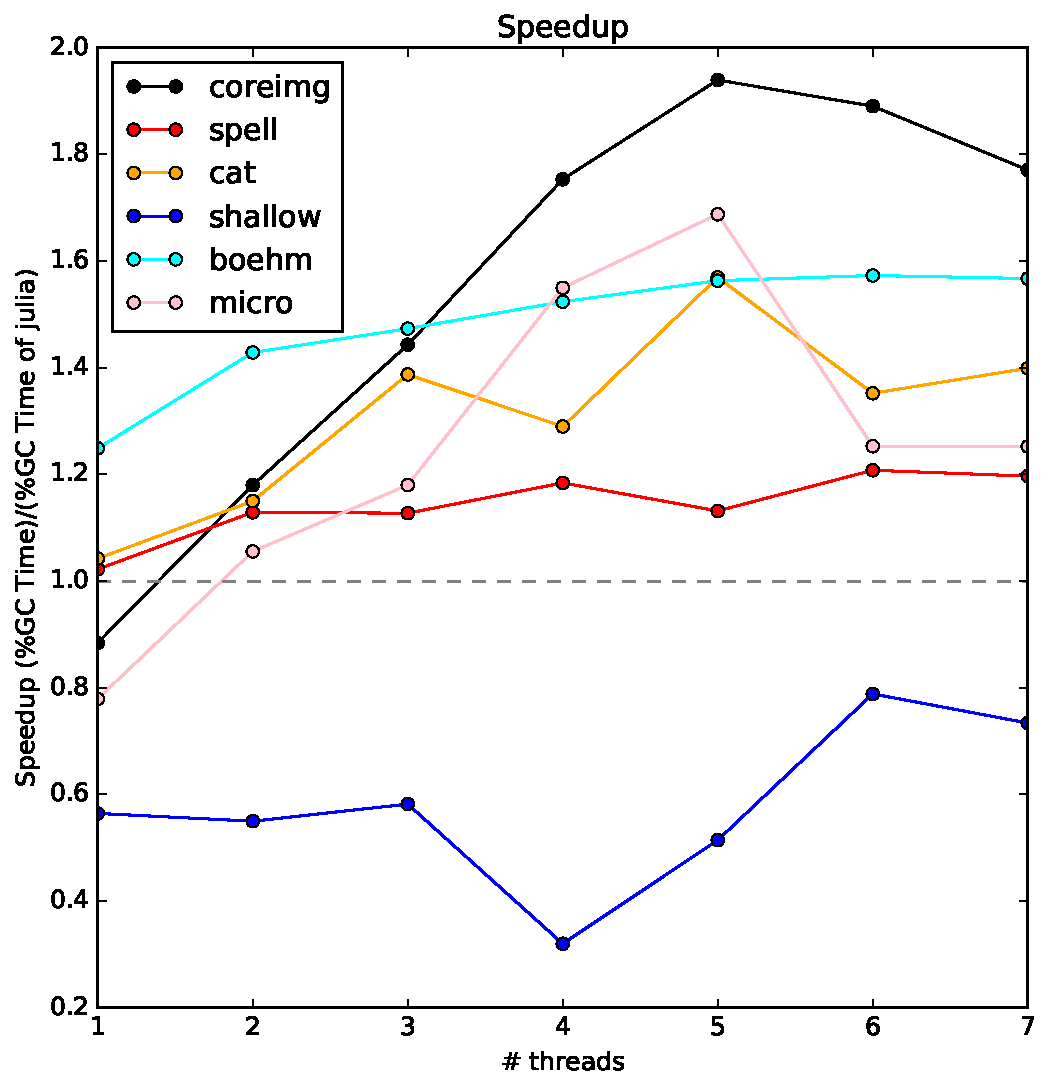
\includegraphics[height=4.8cm]{figures/speedup-julia.pdf}
      \caption{Speedup over Julia}
      \label{fig:speedup}
    \end{subfigure}
    \begin{subfigure}{0.34\textwidth}
      \centering
      % \vspace{-2em}
      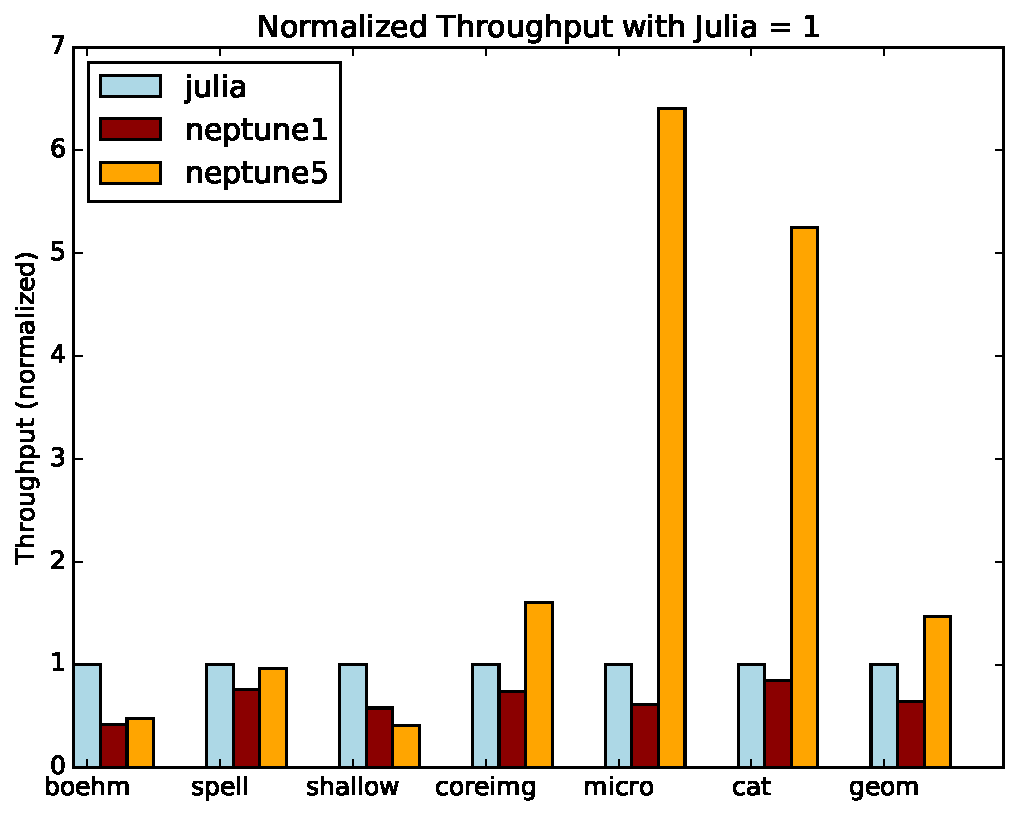
\includegraphics[height=4.8cm]{figures/throughput-normalized-julia.pdf}
      
      \caption{Normalized throughput}
      \label{fig:throughput}
    \end{subfigure}
    \begin{subfigure}{0.34\textwidth}
      \centering
      % \vspace{-2em}
      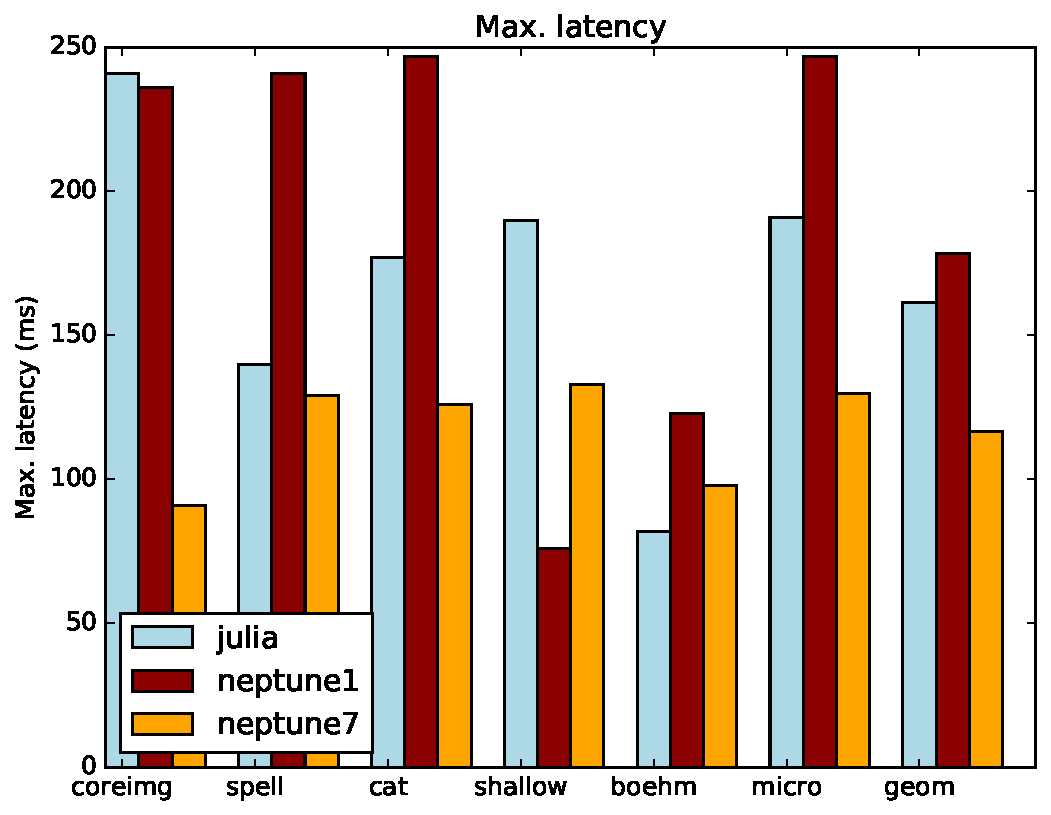
\includegraphics[height=4.8cm]{figures/max-latency.pdf}
      \caption{Maximum GC latency (ms)\\}
      \label{fig:latency}
    \end{subfigure}
    \vspace{-0.5em}
    \caption{Experiment results. Figure~\ref{fig:speedup} shows speedup over Julia in terms of \% time taken in GC normalized with Julia = 1. Figure~\ref{fig:throughput} shows throughput normalized with Julia = 1.}
  \label{fig:results}
\end{figure}

%%% Local Variables:
%%% mode: latex
%%% TeX-master: "report"
%%% End:
